\scanpage{77}
De \unsure{m.|$=$}, on a sur $u(C^{**+})\subset DR^{**+}$ des op.
``puiss. div.'' \inserted{uniques} données par la condition
\[
u(x)^{(i)}=u(x^{(i)})
\]
car il suffit de prouver que si $x'$ est tel que
$ux=ux'$, i.e. $x'=x+y$, $\bar T\cdot y=0$, alors
\inserted{$u(x'^{(i)})=u(x^{(i)})$, i.e. $\bar T_\wedge x'^{(i)}=\bar T x^{(i)}$}
\[
x'^{(i)}=x^{(i)}+x^{(i-1)}y+x^{(i-2)}y^{(2)}-+y^{(i)}
\]
il suffit de prouver que $\bar T y^{(i)}=0$ pour $i\geq1$,
ce qui résulte du fait \deleted{\unsure{évident}}\inserted{que}
\[
\text{\textcircled{D}}\qquad
\inserted{\text{sur}}\quad
\underset{\Vert\,\operatorname{Ker}(\bar T_\wedge(\cdot))}{DR^{**+}}\subset C^{**}.
\quad\deleted{\text{est stable par}}
\quad\begin{gathered}
\text{les puiss. div. (dans }C^{**}\text{)}\\
y^{(i)}\ (i\geq2)\ \text{sont nulles}
\end{gathered}
\]
\deleted{i.e. si $y\in C^{**+}$, $\bar T\cdot y=0\longrightarrow\bar T\cdot y^{(i)}=0\quad\forall i\geq1$,}

(Ceci sera donc visible sur la construction pour $DR_*^{**}\subset C_*^{**}$,
où loc. $y$ est de la forme $\bar Tz$, donc
$\deleted{\unsure{\bar T_\wedge}}y^{(i)}=\bar T^i z^{(i)}$,
qui est donc nul si $i\geq2$.)

\deleted{(\unsure{NB|E}) $\unsure{DR^{**+}}\bar T(\unsure{x\in DR^{p,0}\subset C^{p,1}})\unsure{=0}$}

Ainsi, les seules données supplémentaires sur $C^{**}$ pour
\deleted{définir}\inserted{décrire} les structures habituelles sur $DR^{**}$ sont
\[
(E)\quad\left\{\begin{aligned}
&\text{``multiplication''}\quad
\unsure{DR}^{0,p\deleted{\unsure{+1}}}\times
\unsure{DR}^{0,q\deleted{\unsure{+1}}}\longrightarrow
\unsure{DR}^{0,p+q\deleted{\unsure{+1}}}
\quad(p,q\geq1)\\
&\text{``puiss. divisées''}\quad
\unsure{DR}^{0,p}\xrightarrow{\gamma^i}
\unsure{DR}^{0,pi\deleted{\unsure{+1}}}
\quad(i\geq2)
\end{aligned}\right.
\]
\margin{(\uline{\unsure{données}})}
\deleted{(\uline{NB} \unsure{sur}
$Z^{0,1}\times Z^{0,q+1}-$ pour $p$ ou $q=1$,
$-\unsure{Z^{0,p+q+1}}$ puisque $Z^{0,1}$ est engendré par}
\figure{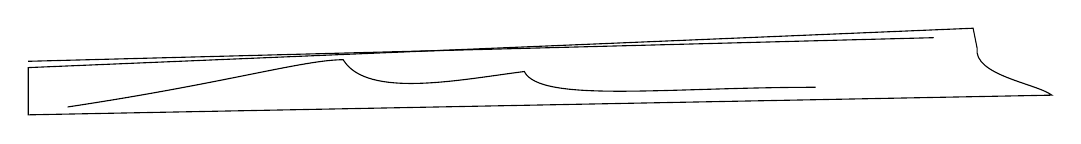
\begin{tikzpicture}
\draw (0,0)--(12,.5)--(12.05,.25) .. controls (12,-.1) and (12.8,-.2) .. (13,-.35)
--(0,-.6)--cycle;
\draw (0,.08)--(11.5,.38);
\draw (.5,-.5)..controls(2.5,-.2)and(3.5,.1)..(4,.1)
..controls(4.3,-.4)and(5.5,-.15)..(6.3,-.05)
..controls(6.5,-.45)and(8.1,-.25)..(10,-.25);
\end{tikzpicture}}
plus les axiomes divers qu'il faut pour assurer que sur $DR^{**}$, on a les propriétés habituelles pour les opérations.
\margin{76}
